%نام و نام خانوادگی:
%شماره دانشجویی: 
\مسئله{پارسر \lr{LR(1)}}
\پاسخ{ }
\\
الف) عکس دیاگرام در زیر قرار داده شده است:
\graphicspath{{./images/}}
\begin{center}
	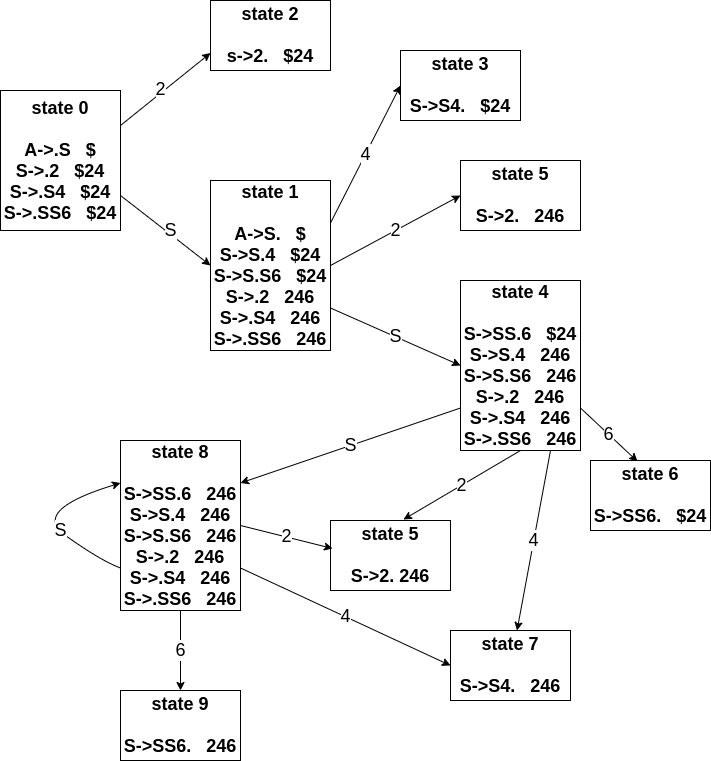
\includegraphics[scale=0.65]{compiler_hw2_q8.png}
\end{center}
ب) عکس جدول در زیر قرار داده شده است:
\begin{center}
	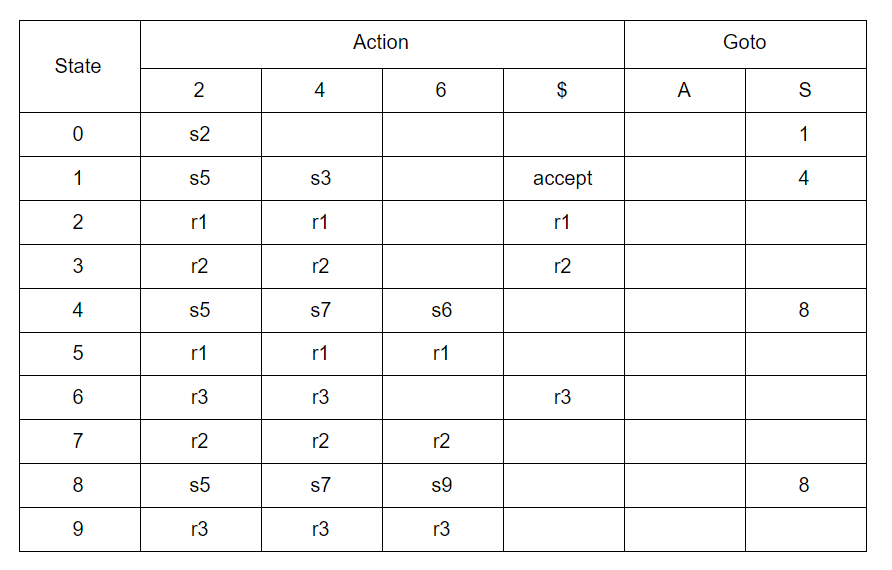
\includegraphics[scale=0.9]{compiler_hw2_q8_table.png}
\end{center}
ج) مراحل ایجاد درخت پارس $226422466$ را در پایین نوشته‌ایم: (دقت شود که حروفی که بین دو | می‌آیند در مرحله بعدی قرار است با هم، به کمک قاعده تولید reduce شوند)
\begin{latin}
	2
	\\
	|2|
	\\
	S
	\\
	S 2
	\\
	S |2|
	\\
	S S
	\\
	S S 6
	\\
	|S S 6|
	\\
	S
	\\
	S 4
	\\
	|S 4|
	\\
	S
	\\
	S 2
	\\
	S |2|
	\\
	S S
	\\
	S S 2
	\\
	S S |2|
	\\
	S S S
	\\
	S S S 4
	\\
	S S |S 4|
	\\
	S S S
	\\
	S S S 6
	\\
	S |S S 6|
	\\
	S S
	\\
	S S 6
	\\
	|S S 6|
	\\
	S
\end{latin}
در نهایت درخت پارس رشته به صورت زیر می‌شود:
\begin{center}
	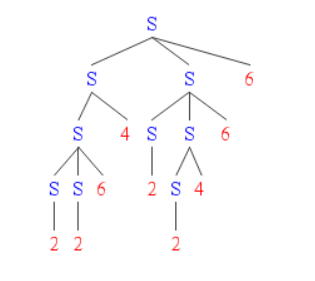
\includegraphics{226422466.png}
\end{center}


